\section{Technische Spezifikationen des Microvision ShowWX+\textsuperscript{\texttrademark}}
\label{app:projector}
\begin{table}[!ht]
\begin{center}
\setlength{\tabcolsep}{20pt}
\begin{tabular}{lr}
\toprule
Eigenschaft & Spezifikation \\
\midrule
Auflösung 	& WVGA (\SI{848}{}$\mathrm{x}$\SI{480}{} Pixel) \\ \addlinespace
Seitenverhältnis & \SI{16}{}$:$\SI{9}{} \\ \addlinespace
Helligkeit 	& \SI{15}{} Laser-Lumen \\ \addlinespace
Wiederholfrequenz & \SI{60}{\Hz} \\ \addlinespace
Farbumfang 	& $\sim$ \SI{200}{}\% NTSC \\ \addlinespace
Kontrastverhältnis 	& $>$ \SI{5}{}.\SI{0}{}\SI{0}{}\SI{0}{}$:$\SI{1}{} \\ \addlinespace
Projektionsverhältnis 	& \SI{1}{}$:$\SI{1}{} \\ \addlinespace
Öffnungswinkel & $\sim$ \SI{30}{°}\\ \addlinespace
Projektionsdistanz 	& \SI{200}{\milli\meter}$-$\SI{2500}{\milli\meter} \\ \addlinespace
Bildgröße 	& \SI{150}{\milli\meter}$-$\SI{2500}{\milli\meter} \\ \addlinespace
Verschlüsselung 	& HDCP \\ \addlinespace
Videoeingang & HDMI (\SI{480}{p}) \\ \addlinespace
Länge & \SI{118}{\milli\meter}\\ \addlinespace
Breite & \SI{60}{\milli\meter}\\ \addlinespace
Höhe & \SI{14}{\milli\meter}\\ \addlinespace
Gewicht 	& \SI{122}{\gram} \\ 
\bottomrule
\end{tabular}
\caption{Technische Spezifikationen des Microvision ShowWX+\textsuperscript{\texttrademark}}
\end{center}
\label{tab:landmarks_f1}
\end{table}

%\begin{figure}[hb]
%\vspace{-5mm}
%\begin{center}
%		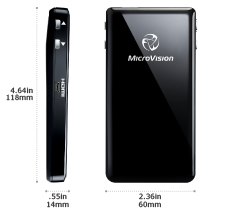
\includegraphics[scale=0.8]{measurements_showwx}
%\end{center}
%\vspace{-5mm}
%\caption{Abmessungen des Microvision ShowWX+}
%\label{fig.specs_proj}
%\end{figure}

\clearpage{}

\section{Technische Spezifikationen des Arduino\textsuperscript{\texttrademark} Nano}
\label{app:arduino}

\begin{table}[ht]
\begin{center}
\setlength{\tabcolsep}{20pt}
\begin{tabular}{lr}
\toprule
Eigenschaft & Spezifikation \\
\midrule
Microcontroller & Atmel ATmega328\\ \addlinespace
Betriebsspannung & \SI{5}{\volt}\\ \addlinespace
Eingangsspannung & \SI{7}{}$-$\SI{12}{\volt}\\ \addlinespace
Grenzen der Eingangsspannung & \SI{6}{}$-$\SI{20}{\volt}\\ \addlinespace
Digitale I/O Pins & \SI{14}{}\\ \addlinespace
Analoge Eingangspins & \SI{8}{}\\ \addlinespace
Gleichstrom pro I/O Pin & \SI{40}{\milli\ampere}\\ \addlinespace
Flash Speicher & \SI{32}{KB}\\ \addlinespace
SRAM & \SI{2}{KB} \\ \addlinespace
EEPROM & \SI{1}{KB}\\ \addlinespace
Taktfrequenz & \SI{16}{\mega\Hz}\\ \addlinespace
Länge & \SI{45}{\milli\meter}\\ \addlinespace
Breite & \SI{18}{\milli\meter}\\ \addlinespace
Gewicht & \SI{5}{\gram}\\
\bottomrule
\end{tabular}
\caption{Technische Spezifikationen des Arduino\textsuperscript{\texttrademark} Nano}
\end{center}
\label{tab:arduino}
\end{table}

\clearpage{}

\section{Technische Spezifikationen des Raspberry Pi\textsuperscript{\texttrademark}}
\label{app:raspberry}

\begin{table}[ht]
\begin{center}
\setlength{\tabcolsep}{18pt}
\begin{tabular}{lr}
\toprule
Eigenschaft & Spezifikation \\
\midrule
System-on-a-Chip & Broadcom BCM2835\\ \addlinespace
CPU & \SI{700}{\mega\Hz} ARM11 ARM1176JZF-S\\ \addlinespace
GPU & Broadcom VideoCore IV\\ \addlinespace
Speicher & \SI{512}{GB}\\ \addlinespace
USB 2.0 Ports & \SI{2}{}\\ \addlinespace
Videoausgänge & Composite RCA, HDMI\\ \addlinespace
Audioausgänge & \SI{3,5}{\milli\meter} Jack, HDMI\\ \addlinespace
Low-Level Peripherie & \SI{26}{} General Purpose Input/Output Pins,\\
& Serial Peripheral Bus Interface (SPI), I²C, I²S,\\
& Universal Asynchronous Receiver/Transmitter (UART)\\ \addlinespace
Netzwerkschnittstelle & \SI{10}{}/\SI{100}{} wired Ethernet RJ45\\ \addlinespace
Stromaufnahme & \SI{700}{\milli\ampere}\\ \addlinespace
Spannungsversorgung & \SI{5}{\volt}\\ \addlinespace
Länge & \SI{85}{\milli\meter}\\ \addlinespace
Breite & \SI{56}{\milli\meter}\\ \addlinespace
Höhe & \SI{15}{\milli\meter}\\ \addlinespace
Gewicht & \SI{31}{\gram}\\
\bottomrule
\end{tabular}
\caption{Technische Spezifikationen des Raspberry Pi\textsuperscript{\texttrademark}}
\end{center}
\label{tab:raspberry}
\end{table}

\clearpage{}

\section{Technische Spezifikationen der inertialen Messeinheit}
\label{app.imu}

\begin{table}[ht]
\begin{center}
\setlength{\tabcolsep}{20pt}
\begin{tabular}{lr}
\toprule
Eigenschaft & Spezifikation \\
\midrule
Chip & MPU-9250 \\ \addlinespace
Stromaufnahme & \SI{3,5}{\milli\ampere} \\ \addlinespace
Spannungsversorgung & \SI{2,4}{}$-$\SI{3,6}{\volt} \\ \addlinespace
Schnittstellen & I²C, SPI \\ \addlinespace
Messbereich Drehrate & \SI{250}{}$-$\SI{2000}{} $\nicefrac{\deg}{\sec}$\\ \addlinespace
Messbereich Beschleunigung &  \SI{2}{}$-$\SI{16}{} $\mathrm{g}$\\ \addlinespace
Breite & \SI{20}{\milli\meter} \\ \addlinespace
Höhe & \SI{22}{\milli\meter}\\
\bottomrule
\end{tabular}
\caption{Technische Spezifikationen der inertialen Messeinheit}
\end{center}
\label{tab:imu}
\end{table}

\clearpage{}

\section{Datenstruktur zur Repräsentation der Modellszene}
\label{app.datastructure}
\begin{lstlisting}[label=source.data,caption=Datenstruktur zur Repräsentation der Modellszene]
<?xml version="1.0"?>
<modelscene>
     <name>Model_World</name>
     <object>
          <name>Map</name>
          <position>
          	<x>0</x>
          	<y>0</y>
          	<z>0</z>
          </position>
          <orientation>
          	<y>0</y>
          	<p>0</p>
          	<r>0</r>
          </orientation>
          <texture>map.jpg</texture>
          <geometry>map.obj</geometry>
          <visible>false</visible>
     </object>
          <object>
          <name>Power_Outlet</name>
          <position>
          	<x>3.15</x>
          	<y>1.8</y>
          	<z>0.4</z>
          </position>
          <orientation>
          	<y>90</y>
          	<p>0</p>
          	<r>180</r>
          </orientation>
          <texture>outlet.jpg</texture>
          <geometry>outlet.obj</geometry>
          <visible>true</visible>
     </object>
</modelscene>
\end{lstlisting}

\clearpage{}

%\section{Bayes Filter}
%\label{app:bayes}
%
%\clearpage{}

%\section{Konstruktionszeichnungen und Modelle}
%\label{app:construction}
%
%\clearpage{}
%
%\section{Launchfiles}
%\label{app:launchfiles}